\chapter{Project development: web application for \\ multimedia editing}
\label{ch:ch3_ProjectDevelopment}

% --- Chapter 3 start ---

This chapter is meant to illustrate the main thesis about the Remix Culture by combining most of the topics presented in the previous parts into a practical example of project development. The project consists in developing a web application for multimedia editing that can run in every modern browser. Hence, from a general point of view this can be seen as an implementation of a set of features that are common in many offline and online tools for video-editing, as analysed in section \ref{sec:stateOfArt} \emph{State of the art: web video-editing tools}. In more detail, the application main value proposition is to offer the possibility of “remixing” different types of multimedia content, in particular videos, images, and sound media. Thanks to this universally accessible and Open Source technical solution the Remix Culture can come to life and can be experienced by anyone with an internet connection.

More details about the requirements, technical decisions and considerations can be found in the paragraph \ref{sec:SoftwareArchitecture} \emph{Project idea and Front End Software Architecture}. At this point, the main argument is addressed from the perspective of software development. Specifically, the results presented in this this chapter follow a two-pronged objective.

Firstly, the development of an application for remixing multimedia enables users to experience the concepts of the aforementioned Remix Culture by enhancing content discoverability and stimulating user’s creativity. On the other side, content holders, i.e., authors, institutions, etc. can gain in recognition, thus receive added value from this kind of application. Therefore, this can be seen as an attempt to promote the Remix Culture among institutions which may be encouraged by the benefits and decide to upload content on the platform. A particularly suitable target might consist of cultural heritage organisations with their frequent digitalization programmes. These institutions’ digitization strategies often set their priority goals for enhancing user engagement and participation.

A second objective comes from the choices made for the technical architecture. The video-editing tool is open for modifications in terms of software development. By publishing and applying the “MIT” license\footfullcite{mitLicense} to the source code, a contribution to the Open Source is made. Furthermore, by adopting a component driven development with a solution based on Web Components technology – a standard and framework agnostic solution as explained in paragraph \ref{sec:webComponents} \emph{Web Components} – the technical solutions are offered to the community as a library from which to choose from, expand upon, and create brand new projects.

In the next paragraph, \ref{sec:reuseAndMaintainability} \emph{Reusability and maintainability, through abstractions to a component-based approach}, an analysis of the modern software development is presented together with arguments in favour and against the adoption of a component-based approach.

Finally, at the end of this chapter, two examples of application instances will be made: the first example was developed in the context of the \emph{PH-Remix} project. In this case, as mentioned in the introduction, the content belongs to the “Mediateca Toscana”\footfullcite{mediateca} and the development was guided by the requirements expressed in the regional project grant. The project involves several researchers, and the development is still in progress as the project deadline is set to 2022. Therefore, a front-end component (or set of components) was implemented, in anticipation of the back end architecture, while work on the latter is still in progress at the time of writing.
The second application integrates a variety of Open Source materials. It is an example of reusability of the components architecture that can be used for different purposes. The implementation is based on the public Pexels API\footfullcite{pexels} which offers a large number of videos and images. All the content can be used thanks to a permissive license. This solution acts as an aggregator of Open Source licensed materials to create new general purpose productions. It is not connected to any specific target audience. An example could be the discovery of content to be used as commercial advertisement for any kind of industrial product.

\section{Reusability and maintainability, through abstractions to a component-based approach}
\label{sec:reuseAndMaintainability}

Modern software development techniques and tendencies are mainly concerned with the objective of simplifying the development of technical solutions, as well as easing up code reusability and maintainability.

Nowadays, programming – the activity of writing a code – involves the use of a growing number of abstractions as a way of responding to the challenges deriving from the complexity of modern software applications. R.C. Martin in the introduction of Clean Code\footfullcite{CleanCode} affirms that:

\begin{displayquote}

“[…] the level of abstraction of our languages will continue to increase. I also expect that the number of domain-specific languages will continue to grow. This will be a good thing. But it will not eliminate code […]”. 

\end{displayquote}

As the author confutes the “no-code development approach”, he also states that the code will be evolving as an expression of the software specifications. These specifications or requirements need to be translated into a form that is understandable and executable by a machine. Hence, the concept of abstractions will be analysed as one of the guiding principles of software evolution.

Focus will be put on the front-end development ecosystem, as it reflects the majority of work done for this dissertation practical application. Despite this choice, most of the arguments presented apply to the software world in general. The final aim of this paragraph is to provide the rationale behind the choice of Web Components as the technology for project development. As a matter of fact, before introducing Web Components, to fully understand the component-based approach, an introspection into the web development stack ought to be made.

The front-end development is commonly considered as a fast-paced environment among developers\footnote{It is worth noting how this statement can be sustained by real world data. Stack Overflow makes yearly surveys among its community of developers. The Stack Overflow Annual Developer Survey (https://insights.stackoverflow.com/survey/) contains a section called “trending techs” where the rise and decrease in popularity of web development technologies over the years can be analysed in further detail}. In short, the lifecycle of the technologies used for the web application layer is shorter compared to the rest of the software world. Consequently, programmers usually need to make a significant effort in order to stay up-to-date on the recent technological progress. In other words, front-end frameworks and libraries tend to become less maintained, and thus deprecated in a short span of time.

Although the fundamental programming skills required for creating web applications – ranging from simple static websites to complex online platforms – are still based on HTML, CSS, and JavaScript, several solutions were created for more efficient and effective way of reaching programming goals. A relevant example of this evolution is provided by JavaScript frameworks and libraries. It is worth emphasizing that JavaScript started off as a scripting language, generally used for small tasks like adding interactivity to the web pages. As of today, it has become a mature and widely used language both on the front-end and the back-end side (mainly thanks to the development of V8 JavaScript engine used for runtimes environments of Node.js, Deno etc.).

On the front-end side, the progress might be viewed as a development of proprietary and Open Source systems that implement features with the goal of easing up and speeding up the development of web projects. Starting from the jQuery library in 2006, which offered a cross-browser compatible set of features with an API that simplified the most frequent actions like DOM traversal, event handling etc., to the first frameworks (Backbone, Ember, Angular just to name a few) with more sophisticated features like data binding, dependency injection, routing and many more. Another popular, more recent example is the React library.

One of the core innovations of the React library is its design principle of “composition of components”. This principle consists in building “encapsulated components that manage their own state, then compose them to make complex UIs”\footfullcite{reactDesignPrinciple1}. This innovation, as seen in React, reflects the tendency of many other modern front-end frameworks, such as: Vue, Angular, Svelte, etc. They are based on the idea of splitting codebases into small reusable pieces of code, called components. This approach is particularly useful for medium and large software projects as it enables modularization, by splitting software logic into separate modules, thereby encouraging reusability and maintainability. Another benefit of this approach is that the development process can also be better organised between multiple teams working on different features. 

As more and more solutions were introduced into the web development ecosystem, a phenomenon commonly called “proliferation of frameworks”\footfullcite{proliferationFrameworks} became an issue. An issue that might have consequences beyond the vastity of the offer to choose from.
An immediate consequence of using frameworks is the framework-specific way of developing code or components. The developers are required to learn a new framework and dedicate to it in order to gain the benefits that are being offered by those solutions. A flaw of this approach logically follows as the development becomes limited to the specific framework or technology. It seems that more arguments on the downside of using frameworks can be made. The possible common issues involve their lifespan and changes due to new releases that may lead to issues with compatibility between the old and the new versions. Also, the size of the framework codebase, i.e., the functions installed and required by default – often not necessary in every project – can slow down the application performances.
For some projects this might be a viable solution, as for companies currently developing solutions that might benefit from specific features and differences offered by frameworks or for those who can avail of having an internal expertise to justify the usage of a specific framework.

Many of these new features offered by the above tools are connected to the standardization process itself. It seems that the creation of new solutions that gain popularity within the community stimulate the implementation of these features into web standards. Notably, in this context, W3C recommendations standards\footfullcite{w3c} and JavaScript ECMAScript specification \footfullcite{ecma}. Arguments in favour of this thesis can be made. For example, the standard Selectors API specification\footfullcite{w3cSelectors}, offering “querySelector” “querySelectorAll” interfaces for finding elements inside the DOM tree structure, was inspired by the jQuery selectors helper methods\footfullcite{jQuerySelector}. From the perspective of frameworks or libraries adopters the benefits of adopting the libraries over the native standard – which is faster – are inversely proportional to the number of features that exist in the standard. Although nothing prevents developers from adopting jQuery and similar solutions, their adoption may make less and less sense leading to their natural decline.

This prompts the question, if the component approach seems to be a shared direction for developing more complex front-end systems, how to tackle the issues regarding supposedly one of the main features of components, namely the benefit of writing a reusable code while being locked-in into specific technology stacks?

A possible answer might be in the Web Components technology which enforces the property of reuse among applications. In short, having a standardized way of building components would mean greater reusability, configurability, and consistency – avoiding technical lock-ins – for many years to come. As a general rule of thumb, Web Standards, made by W3C and similar, are more reliable than the proprietary Long Time Support (“LTS”) solutions. Web components are a set of Web APIs that allow to create custom, reusable HTML elements with logic and styling encapsulated into their definition. They can tackle the problems of developing interoperable components. By inserting the components within the frameworks, they are expected to work in a plug and play manner thanks to the native APIs compatibility\footfullcite{customElementsEverywhere}.

Nevertheless, Web Components are not to be considered a silver bullet for solving issues presented in this section. Currently, it appears that some problems could also be mitigated by adopting a set of techniques and strategies such as “Micro-Frontends”\footfullcite{microFrontends}. The latter combined with “Webpack Module Federation” seems a particularly promising solution. A detailed analysis is beyond the scope of this dissertation. However, for a better perspective of the current state of art, the idea of Micro-Frontends could be summarized as the application of microservices architecture to the front-end world. As it happens with the back-end, the aim is to decouple the single pieces of an application in a way that they can be developed independently and using different technologies. From a business point of view, this would make sense in large projects and is a promising approach to Agile methodology as small teams could work on developing autonomous features. The key difference between the Web Components approach and the Micro-Frontends is that the development of interoperable components can be done by using different frameworks. A quick example could be a coherent application composed by components made with the Vue, React and Svelte frameworks. Certainly, this leads to complexities. Therefore, the Webpack Module Federation was introduced. This Webpack feature allows a JavaScript application to dynamically load code from another application without compromising security\footfullcite{webpack5}.

In this panorama, the Web Components technology seems like an additional asset to the current way of developing front-end projects. Its aim does not involve replacing the actual front-end frameworks, it should rather be considered as one of the possible ways for adopting a component-based approach on the web. 

Returning to the \emph{PH-Remix} case study, the Web Components were adopted as a front-end technology in line with the project architecture. As a matter of fact, the project architecture is based on a microservice model that allows for a degree of flexibility and enables a parallel development of the back-end infrastructure. Also, from the project development point of view, relying on the standard allows for future developers to modify and enrich the code more easily. Consequently, the necessity of learning new frameworks is absent. This suggests that the features that Web Components offer could solve some of these problems. Indeed, the main promise of making a flexible architecture seemed to be easily solved thanks to this front-end technology of choice. In the next paragraph the main standard’s features will be introduced. 

\section{Web Components}
\label{sec:webComponents}

To reiterate the definition from the last paragraph, Web components are a set of Web APIs that allow to create custom, reusable HTML elements with logic and styling encapsulated into their definition. From a practical point of view, modern browsers can compute Web Components in the form of custom HTML tags that, in turn, can be used and re-used across multiple projects and technology stacks. The described behaviour is equivalent to the one of standard HTML elements as defined in the HTML documentation.

Web Components offer a native platform and a technology agnostic component model for developing a code that runs in browsers. As a matter of fact, this follows the tendency of many modern front-end frameworks, which are based on the idea of splitting codebases into components, as mentioned in this chapter’s introduction. The main difference is the interoperability provided by adopting the solution introduced in this chapter.

Web Components technology can be considered as an umbrella term that encompasses three distinct Web APIs: Custom Elements, Shadow DOM, and HTML Templates. By defining and referring to Web Components as a native technology, the standardization by W3C is intended. The specifications for each of these Web APIs are now incorporated as a living standard\footfullcite{w3cEvergreenStandards}. Each of these specifications will be explored with more detail in the next sections to explain their features and the current limits of this technology. The purpose of these explanations is to provide some basic knowledge about the internal mechanisms and a few points of interest relevant to the subject that might be of interest for readers.

The formal documentations and technical definitions hardly give the developer’s perspective and community feelings about this topic. Therefore, another aspect worth investigating regards the evolution and the adoption of Web Components.

The proposal of Web Components is not new, speaking in terms of software development dynamics. Firstly introduced in 2011 by Alex Russell\footfullcite{webComponentsBeginning}, it went through years of standardization process. The latter might be also viewed as search for consensus between browsers producers, namely the owners of: Safari, Firefox, Chrome – therefore, all the Chromium based browsers – and Microsoft browsers. While the Microsoft browsers consist of Internet Explorer and Microsoft Edge, the former has reached the end of its lifecycle maintaining only the technical support and security updates for its latest version (Internet Explorer 11). The browser does not support the Web Components standard\footfullcite{canIUseComponents}, therefore its implementation and usage require the adoption of polyfills and transpilers.
Generally, transpilers are used to compile the source code written in one language to another. Although in this case their main usage is to transform the code written using some – usually recent – standard into a backward compatible code that can work with the old browsers not supporting that standard. One example of the most popular transpiler is Babel\footfullcite{babel}, which allows developers to use the most recent JavaScript features among all the browsers by translating them into a code compliant with the old language standards.


Returning to the issues of browser compatibility, the deprecation of Internet Explorer and the subsequent evolution of its successor, Microsoft Edge, gave Web Components a boost in terms of compatibility. The main reason can be linked back to the Microsoft Edge passage to the Chromium Open Source project on 8th April 2019\footfullcite{microsoftEdge}. This fundamental change consisted in a passage from the combination of EdgeHTML browser engine and Chakra JavaScript engine to Blink and V8, respectively a browser engine and a JavaScript engine.

This led to a substantial improvement and larger adoption by the community. However, this overview draws attention to the standardization process. As seen, almost ten years were necessary until one of the last major browsers adopted the initial proposal. In the meantime, the standard itself came through a long process of maturation and stabilisation\footnote{An interesting lecture by Jan Miksovsky on how the standardization of HTML slot element may give a better view on the complexities of standardization process: https://component.kitchen/blog/posts/a-history-of-the-html-slot-element}.

The longevity of the process exemplified above might imply and justify the existence of critiques against the Web Components standard. By investigating the most common reasons, it appears that they were mainly concerned with cross-browser discrepancies, partial standard adoption, and frequent API changes. Serhii Kulykov, a developer currently working at Vaadin – a company which uses Web Components with an Open Sourced web application platform – critically reviews in his series of blogs\footfullcite{devToWC1}\,\footfullcite{devToWC2} about Web Components and gives an insight view regarding most of the problems previously mentioned.

To summarize, Web Components became standardised and supported by all the major browsers only recently. This suggest that their popularity and adoption rate could lead to a more substantial increment within the web technology market share in the future. Consequently, attracting more developers, who develop more tools leading to possible improvements of the standard itself, as argued above when talking about the connection of standardization and external solutions development. Ultimately this could lead to a substantial front-end innovation.

Looking at the state of art adopters, ING\footfullcite{ing}, AXA\footfullcite{axa} and IBM\footfullcite{ibm} are three examples of companies that implement and Open Source their design systems based on Web Components. Various other components implementations are also present in some of the biggest websites. For example, just to name a few: GitHub, YouTube, Google Earth are among the adopters of Web Components. Especially, Google with its Web Components library, called LitElement, seems committed to the technology. In paragraph 3.3 \emph{Web Components libraries} a more extensive analysis of LitElement will be presented.

As seen up to this point, the overview of state of the art highlights some of the challenges and opportunities for future Web Components development. Before delving into an overview of the WebAPIs technicalities, an introduction to JavaScript Modules will be presented in the following paragraph.

\subsection{JavaScript Modules}
\label{subsec:jSModules}

JavaScript modules (also known as “ES Modules” or “ECMAScript Modules”) are core to the modern web development and can be considered as a prerequisite for the Web Components technology. The definition of a module seems to be quite consistent across the subject literature. A module can be defined as: “[…] a piece of program that specifies which other pieces it relies on and which functionality it provides for other modules to use (its interface)”\footfullcite{EloquentJavascript}.

From a general point of view, modules act as a glue connecting components or code dependencies and therefore allowing for code splitting and composition. This implies the advantage of writing and maintaining a code structure that can be both understandable and maintainable. This can be particularly beneficial for developers (usually people who did not create the original code). Most likely, without modularization, code would be destined to become exponentially complex to organise in relation to the growth of project features.
As written in the “Modules” chapter of “Eloquent JavaScript” book:

\begin{displayquote}

“The phrase “big ball of mud” is often used for such large, structureless programs. Everything sticks together, and when you try to pick out a piece, the whole thing comes apart, and your hands get dirty.”\footfullcite{EloquentJavascript}

\end{displayquote}

This quote resembles the “Tar Pits” metaphor as seen in chapter \ref{ch:ch2_ProjectManagement} \emph{Project Management and interdisciplinary works}, when talking about some of the most common causes leading to failures of software projects from the managerial perspective. Here, the author makes arguments in favour of spending additional time for planning and coding structuring phases. A relevant example might come from the experiences and feelings of many developers who worked or are working with structureless or badly structured code. It may often appear that rewriting code from scratch could be easier than trying to extract it from its original context. 
By joining these two evocative concepts, “big ball of mud” and “tar pits”, a step forward in the direction of project quality improvement can be made. This would mean recognising and preventing the root causes leading to the negative symptoms described above. A possible solution may come from an appropriate combination of good programming practices and management skills.

In 2015 JavaScript introduced its own standardized module system, called ES Modules\footfullcite{mdnModules} with its own import-export syntax. Since 2018 the JavaScript Modules standard is supported by all the major browsers natively\footfullcite{canIUseEs6Module}. Nowadays, this is standard but initially the Web Components technology used to have a fourth element, HTML imports\footfullcite{mdnImports}. The latter was intended as a packaging mechanism for including HTML documents inside other HTML documents. However, the standardization attempt failed since the browser vendors decided not to support it.

A simple example of ES Modules usage logic can be seen in the next code snippet. Assuming the following file structure as proposed in Code \ref{codeModules}.
\\
\begin{lstlisting}[caption={File structure with a module},label={codeModules}, language=JavaScript]
index.html
main.js
modules/ // directory
    utils.js
\end{lstlisting}

In this example one of the functions defined in the file “utils.js” is used inside “main.js” script. This is done by exporting functionality from the module and importing it inside the script thanks to “import” and “export” statements:
\\
\begin{lstlisting}[caption={Import, export directives},label={codeImportExport}, language=JavaScript]
// main.js
import { create } from "./modules/utils.js";

const element = create (document.body, "article-segment");

// utils.js

const MEDIA_TYPES = {
    VIDEO: "video",
    AUDIO: "audio",
    IMAGE: "image"
}

function createAndAppendParagraph(parent, className) {
    let paragraphElem = document.createElement("p");
    paragraphElem.classList.add("${className}");
    parent.appendChild(paragraphElem);
}

export { MEDIA_TYPES, create }
\end{lstlisting}

The code above exports two types of variables, a constant “MEDIA\_TYPES” and a function “createAndAppendParagraph”. In this way any JavaScript construct can be exported if it is not a top-level item, that is: an item not nested inside objects or functions etc. The main script imports one of the exported functionalities, namely the “create” function. The latter is called within “main.js” and appends a DOM HTML paragraph to the parent (passed through the “parent” parameter”) with the class as specified in the “className” parameter. By analogy, the constant “MEDIA\_TYPES” could be imported by an indefinite number of JavaScript scripts. For example, since JavaScript does not implement an “enum” data type it could be used for the purpose of simulating immutable data through code.
In this perspective, modules are crucial for Web Components. Starting from how custom elements are instantiated into an HTML document via the import directive to the inner dependencies between components. Modules allow to avoid conflicts in the global JavaScript namespace, where components could interfere with one another (a concept that will be further extended in section \ref{subsec:shadowDOM} \emph{Shadow DOM}).

By expanding upon the idea of reusability, Web Components should enable developers to pick and use components created from anyone and to incorporate them into their own projects. Indeed, components in general should work like LEGO blocks. Since a Web Component may rely on other Components to work, the modules system provides the mechanism to connect or “glue” everything together in an organised manner. This resolves the “big ball of mud” software problem.

Finally, it might be argued that modularization is crucial for most good practices of software development. Principles like those introduced by Robert C. Martin, commonly called: “SOLID Design Principles”\footfullcite{wikiSolid} but also other principles with rather fascinating acronyms like: DRY\footfullcite{wikiDRY}, KISS\footfullcite{wikiKiss} and YAGNI\footfullcite{wikiYagni} can be thought as a developer’s Swiss Army knife (as a positive metaphor for usefulness and adaptability) for solving present and future software problems. From the web developer’s perspective this may suggests a more efficient and productive way of working. Continuing this tendency of beneficial features in the next paragraphs Web Components APIs will be presented.

\subsection{Custom Elements}
\label{subsec:customElements}

Custom Elements, as defined in the W3C living standard\footfullcite{w3cCustomElems}, can be introduced as: “A set of APIs that allow you to define custom elements and their behaviour, which can then be used as desired in your user interface”\footfullcite{mdnWC}.

From a practical perspective, Custom Elements enable to programmatically extend the base HTMLElement\footfullcite{mdnHTMLElem} (an interface that represents any HTML element) via a Custom Registry API\footfullcite{mdnCustomElemRegistry}. Hence, calling the “CustomElementRegistry” method “define” allows to define a new custom element as demonstrated in the Code \ref{codeCustomElem} \emph{Custom Element definition}. This turns out to be a powerful combination for enriching the HTML native vocabulary of elements with custom tags containing encapsulated functionality.
\\
\begin{lstlisting}[caption={Custom Element definition},label={codeCustomElem}, language=JavaScript]
class VideoEditor extends HTMLElement {
    constructor() {
        super();
        // Some element functionality here
        ...
    }
}
window.customElements.define("video-editor", VideoEditor);
\end{lstlisting}

Custom Elements are created by using the JavaScript class syntax which enables inheritance through the “\emph{prototypal chain}” from HTMLElement interface. In the above example, the code in line 8 registers a Custom Element named “video-editor” (a dash is required by the syntax) whose definition is contained in the class “VideoEditor”, that in turn defines the element’s behaviour.
From now on, the “video-editor” Custom Element can be used just as any other native HTML tag.
\\
\begin{lstlisting}[caption={Custom Element usage},label={codeCustomElemUse}, language=HTML5, numbers=none]
<video-editor></video-editor>
\end{lstlisting}

As mentioned, the class syntax is used to extend the native HTMLElement interface through inheritance. Figure \ref{fig:HTMLInheritance1} \emph{HTML Element Interface} depicts the native hierarchy of Browser APIs.

\begin{figure}[H]
\centering

\includegraphics[width=1\textwidth]{images/HTMLElement - Web APIs MDN.png}
\caption{HTML Element Interface (from Mozilla Developers Network, licensed under CC-BY-SA 2.5)}
\label{fig:HTMLInheritance1}
\end{figure}

In this context, the result of registering the custom element could be viewed as in Figure \ref{fig:HTMLInheritance2} \emph{DOM Inheritance}.

\begin{figure}[H]
\centering
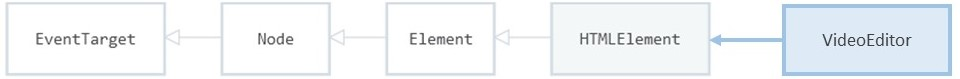
\includegraphics[width=1\textwidth]{images/inherit.jpg}
\caption{DOM Inheritance}
\label{fig:HTMLInheritance2}
\end{figure}

In this way a new \emph{"Autonomous Custom Element"} was created. As seen in the examples, these are elements that do not directly inherit from other elements in the HTML vocabulary (apart from the HTMLElement root). As a matter of fact, the API allows to create two types of custom elements. The second type is called \emph{“Customized built-in element}”, meaning that the custom element extends a built-in HTML element. For example a HTML "p" tag, standing for a paragraph element or the HTML “img” tag standing for image element, and so on.
At the time of writing, the Customized built-in elements have a slightly more limited browser support\footfullcite{canIUseCustomElems}. Furthermore, in this work only Autonomous Custom Elements were used. 

Another important feature of Custom Elements are lifecycle hooks. These hooks – or more precisely, callback functions – can be defined in the class constructor and are automatically executed when elements enter one of the following states\footfullcite{googleWC}:

\begin{itemize}
\item connectedCallback: when the element is appended for the first time into a document’s DOM.
\item disconnectedCallback: when the element is removed from a document’s DOM.
\item adoptedCallback: when the element’s is moved to a new document.
\item attributeChangedCallback: when the element’s attributes are added, removed, or changed.
\end{itemize}

A frequent usage example can be made by considering Custom Element initialization and the update phase. The former triggers a connectedCallback method. Within this method, an initial state of the Component can be set: namely, API calls to populate the User Interface, registration of event handlers etc. Later an update phase can occur when one or more Component attributes change thanks to the attributeChangedCallback method. This is the case of reacting to user actions such as form actions, resolution changes, various interactions on interactive elements and so on. These changes can be automatically captured and reflected dynamically thanks to Component attributes. For example, if users interact with a server, the application state could change. A common scenario is generating a loading state. While the application is waiting for the server response, it can generate the appropriate feedback (a spinner element, helpful text messages etc.).

\subsection{Shadow DOM}
\label{subsec:shadowDOM}

Shadow DOM API as referred in the standard, can be defined as: 

\begin{displayquote}

“A set of JavaScript APIs for attaching an encapsulated "shadow DOM” tree to an element — which is rendered separately from the main DOM document — and controlling associated functionality”\footfullcite{whatwgSD}.

\end{displayquote}

In other words, it enables to attach a separate, encapsulated DOM which is isolated from the rest of the page. This is particularly useful for Custom Elements. It implies that the functionality defined inside a component, i.e., styles, markups and behaviour is limited (encapsulated) within the Shadow DOM boundaries. In other terms, anything happening inside a Shadow DOM does not have any effect outside of it.

The Shadow DOM API method, “attachShadow”\footfullcite{mdnShadow} is used for attaching a Shadow DOM to an HTML Element (therefore any\footnote{Shadow DOM cannot be attached to every HTML element, a list of HTML element supporting this functionality can be found in the documentation.} autonomous custom elements defined in the previous section).

The consequences can be seen with an example. Given two components: “Component A” and “Component B”, supposedly both containing an HTML input element with an attribute, “id” set to value “input-1”. Standing to the HTML best practices “ids” should be unique in the entire document. This is not the case of this example as “Component A” DOM is fully separated from “Component B” DOM. Therefore, elements referred by the id “input-1” can be styled and referenced separately for the two components even if they were instantiated inside the same application.

Code \ref{codeShadowDOM} shows the shadow DOM attachment to a standard HTML Element and a Custom Element.
\\
\begin{lstlisting}[caption={Shadow DOM attachment},label={codeShadowDOM}, language=JavaScript]
// Shadow Root attachment to HTML <article> element
const htmlInput = document.createElement("article")
        .attachShadow({ mode: "open" });

// Shadow Root attachment to Custom Element
class VideoEditor extends HTMLElement {
    constructor() {
        super();
        // Some element functionality here
        ...
        this.attachShadow({ mode: "close" });
    }
}
\end{lstlisting}

The Shadow DOM API allows to attach two types of Shadow DOM. An open shadow root allows accessing the DOM outside of the HTML element definition while a closed shadow root does not expose the DOM outside of the element. In the latter case the DOM cannot be referenced and accessed outside of its context. In theory, it exists in the flow of the document since it is rendered but its functionality is hidden from the rest of the page. However multiple ways of “hacking through” the limitations of closed shadow root exist\footfullcite{ShadowDomBlog}, therefore the usage of open shadow DOMs is recommended.

Finally, an overview to summarize the concepts introduced can be seen in Figure \ref{fig:shadowDom}: \emph{DOM Tree and Shadow Tree}.

\begin{figure}[H]
\centering
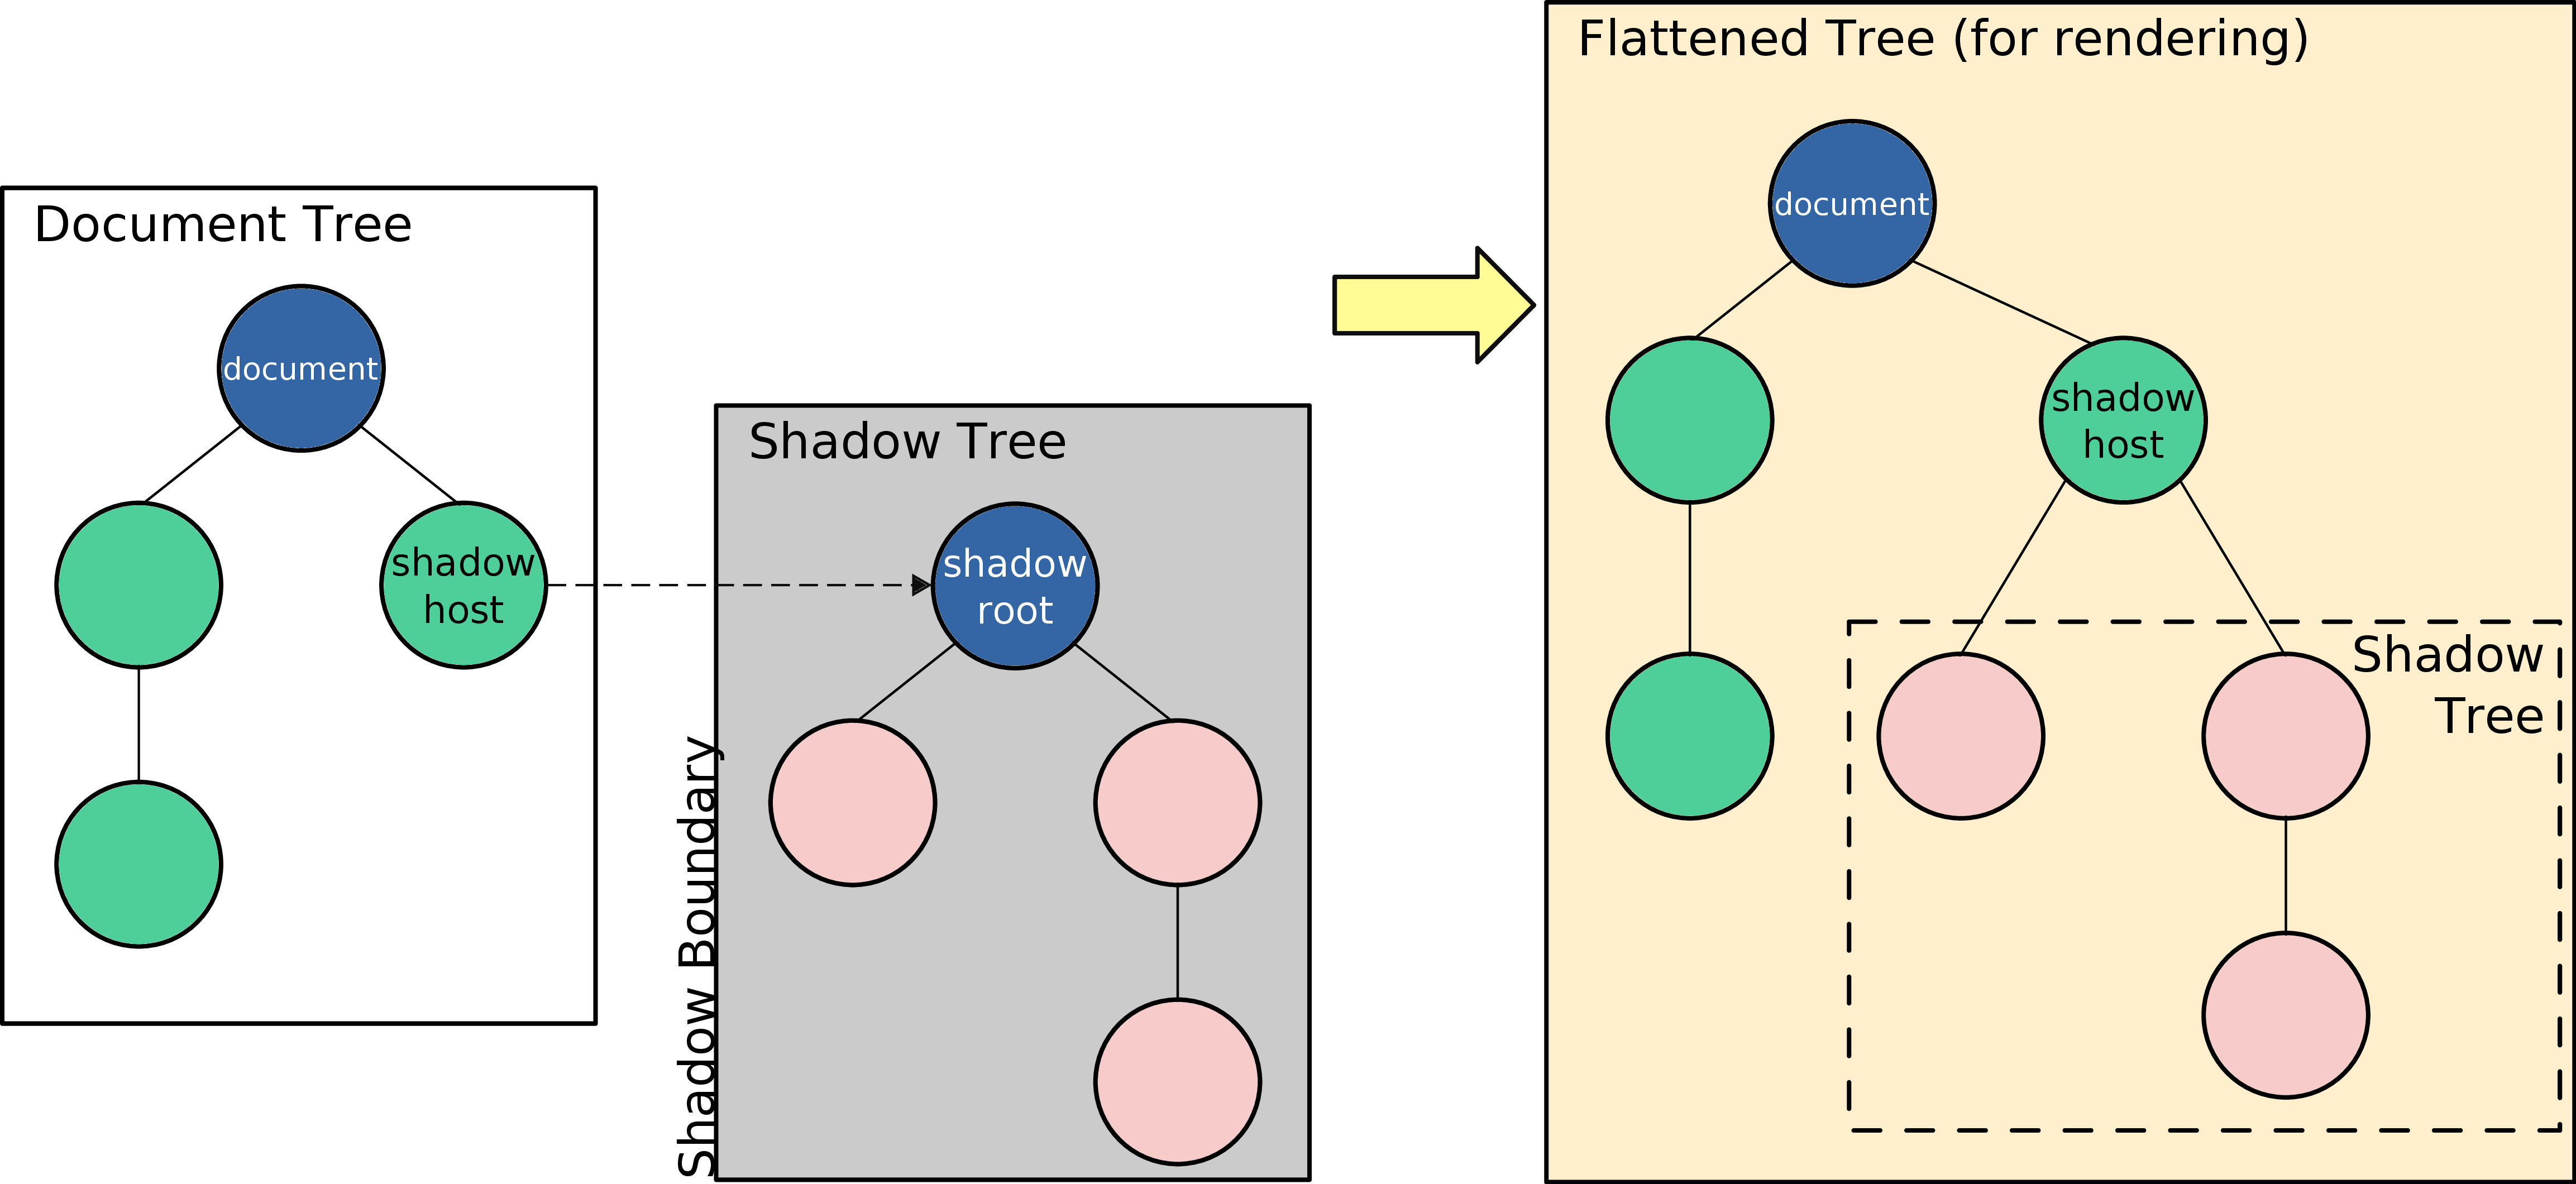
\includegraphics[width=1\textwidth]{images/shadowdom.jpg}
\caption{DOM Tree and Shadow Tree (from Mozilla Developers Network, licensed under CC-BY-SA 2.5)}
\label{fig:shadowDom}
\end{figure}

Some basic terminology is also explained in the documentation\footfullcite{mdnUsingShadow}:

\begin{itemize}
\item Shadow host: The regular DOM node that the shadow DOM is attached to.
\item Shadow tree: The DOM tree inside the shadow DOM.
\item Shadow root: The root node of the shadow tree.
\item Shadow boundary: the place where the shadow DOM ends, and the regular DOM begins.
\end{itemize}

\subsection{HTML Templates}
\label{subsec:HTMLTemplates}

The HTML Templates technology consists of HTML template\footfullcite{whatwgTemplate} and HTML slot\footfullcite{whatwSlot} elements, specified by the W3C living standards. Among the main characteristics, they allow to produce reusable content that can be defined, referenced by JavaScript, and later instantiated inside the DOM Document. This can be useful for creating content with redundant structure only once.

The Template element “is a mechanism for holding HTML that is not to be rendered immediately when a page is loaded but may be instantiated subsequently during runtime using JavaScript”\footfullcite{mdnTemplate}. This definition suggests that HTML structures of arbitrary complexity can be created and dynamically appended to the DOM Document.
\\
\begin{lstlisting}[caption={HTML Template creation},label={htmlTemplate}, language=HTML]
<template class="image-gallery">
    <ul class="gallery-list">
        <img src="firstImage.png" alt="first image description">
        <img src="secondImage.png" alt="second image description">
    </ul>
</template>
\end{lstlisting}

Notably, this approach can be used with and within Web Components to produce templates of components. Therefore, components can be put inside templates and instantiated when and where necessary.
While templates are a more general purpose mechanism, the slot element was introduced specifically for the Web Components technology context.  Thanks to the “slot” tag, developers can create placeholders inside Web Components that allow to instantiate additional children with their own separate DOM trees. Compared to templates, slots offer greater flexibility and configurability (intended as the possibility of instantiating dynamically generated markup). By expanding upon the last example, it should be possible to visualize how slots enable greater flexibility.
\\
\begin{lstlisting}[caption={Slotted templates},label={slottedTemplate}, language=HTML]
<template class="image-gallery">
    <ul class="gallery-list">
        <slot name="image-description"></slot>
        <img src="firstImage.png" alt="first image description">
        <slot name="image-footer"></slot>
        ...
    </ul>
</template>
\end{lstlisting}

From now on, any valid HTML element can replace the slot placeholders by referring to their name attribute (indeed, they can also be called “named slots”). A paragraph with an image description can be expected on top of the "img" element, also a footer containing the author’s credits and a hyperlink to other similar work can be imagined.

This procedure allows for greater reuse of specific parts of markup, the latter can be instantiated differently depending on the context. Another example comes from the work done for this dissertation project. The Query-Text Web Component – in practice a search bar – can be optionally instantiated with a “slottable” button coming from an external Web Components library with its own Shadow DOM and encapsulated behaviours (figures: \ref{fig:queryTextBase} \emph{Query-Text base class} and \ref{fig:queryTextSlotted} \emph{Query-Text with slotted search button} demonstrate these differences).

Overall, templates and slots in conjunction allow for a powerful composition of markup, thus preventing redundancy and shortening the code. 

\section{Web Components libraries}
\label{sec:wCLibraries}

Web Components libraries were created with the main intent of simplifying and speeding up the development process. Libraries usually provide some sort of abstractions on top of the native Web Components for efficiency and in order to enable new features.

During the planning phase, some of the most popular and active Web Components libraries were considered for adoption: LitElement\footfullcite{lit}, FAST\footfullcite{fast}, hybrids\footfullcite{hybrids}, Stencil\footfullcite{stencil} and Adobe Spectrum\footfullcite{spectrum}.
By looking at these proposals and the companies behind each library, it emerges that some important organisations are investing in and actually using the Web Components technology. Namely, FAST is authored by Microsoft, LitElement by Google, Adobe by Adobe, and Stencil is made by the Ionic Framework team\footfullcite{ionic}. Hybrids is an exception since it is a community based effort.

As anticipated, LitElement was the choice for the dissertation’s project. It originated from Google’s Polymer library. This library was mainly chosen due to its popularity, the presence of a large and thriving community involved in the project and a high quality exhaustive documentation\footfullcite{litDocs}. Certainly, the features offered and the fact that LitElement is fully compatible with all the browsers which adopt the native Web Components technology was also crucial during the decision making process.
Indeed, LitElement is an abstraction over the native HTMLElement. By using LitElement class-based components, developers are extending the LitElement class which in turn extends HTMLElement behind the scenes.

LitElement provides features like reactive state, scoped styles, and a declarative template system that are extensively used during this project’s development. The former can also be defined as reactive properties, i.e., properties that hold the state of the component. This implies that changing one or more of the components' reactive properties automatically triggers an update cycle, re-rendering the component. From the developer point of view this is a big simplifier. Indeed, by combining another LitElement feature, declarative templates, the User Interface can be efficiently updated and almost without writing any code.

Lit templates allow to render dynamic contents thanks to many helper operators. As stated in the official documentation\footfullcite{litTemplates}:

\begin{itemize}
\item Expressions: Templates include dynamic values called expressions that can be used to render attributes, text, properties, event handlers, and even other templates.
\item Conditionals: Expressions can render conditional content using standard JavaScript flow control.
\item Lists: Render lists by transforming data into arrays of templates using standard JavaScript looping and array techniques.
\end{itemize}

Finally, thanks to the scoped styles feature, LitElement automatically attaches a Shadow DOM to the component. This allows to define encapsulated styles that affect only the components context.

\section{Project idea and Front End Software Architecture}
\label{sec:SoftwareArchitecture}

In this section, a brief discussion about the project idea and its evolution will be introduced followed by a description of the adopted front-end software architecture. As mentioned in this work’s introduction, the application idea was originated from the activities related to the \emph{PH-Remix} interdisciplinary project.

The practical project work of this dissertation is mainly concerned with the development of an in-browser multimedia editing tool. This tool – called “Remix environment” or “Remix platform” in the \emph{PH-Remix} context – allows for discovery and reuse of multimedia content.

Two phases of development can be extrapolated from a temporal perspective. In the first phase, the application was subject to goals and requirements defined for the \emph{PH-Remix} project. In the second phase, the application was expanded upon to fit a more general scenario. These two phases ought not to be considered as mutually exclusive. On the contrary, thanks to modularity and configurability, the application can accommodate the requirements of the \emph{PH-Remix} project as well as alternative project ideas and implementations. The latter point might be viewed as particularly interesting in the context of this work’s narrative. By demonstrating that multiple applications can be made using the same components it seems that a remix can be applied to the software world. The components can be assembled like LEGO blocks alongside with other components developed from the community, an argument best exemplified in paragraph \ref{sec:appExamples} \emph{Examples of applications}.

The first step of this work involved defining an appropriate software architecture and was done thanks to the collaboration with the \emph{PH-Remix} project members. Consequently, the project was initialized with the subsequent goal of producing an application prototype. The prototype can be seen as an evolutionary prototype\footfullcite{wikiPrototyping} due to the adopted architecture that can be easily refined and expanded.

The front-end architecture was driven by the principles of microservices architecture\footfullcite{redHat}. Namely, the Web Components technology is used as foundation for adopting the separation of concerns design principle\footfullcite{wikiSoc} between application components. The main choices for the adoption of Web Components adoption were made by keeping in mind the benefits of flexibility, maintainability, and scalability. Also, for the sake of efficiency and productivity LitElement was adopted as the Web Component library.

The core front-end structure is composed of the following components: 

\begin{itemize}
\item Video-Editor-App
    \begin{itemize}
        \item Video-Preview
        \item Track-Editor
    \end{itemize}
\item Query-Ui
    \begin{itemize}
        \item Query-Text
        \item Result-Media
    \end{itemize}
\end{itemize}

As seen in the list above, two components’ levels can be distinguished. On the top-level, the Video-Editor-App and Query-Ui act as wrappers. They can instantiate the components below. They are designed for managing the communication between the client side and the server side through API calls. Therefore, they are more project specific – than the components at one level below – and must be configured in order to request and retrieve application specific data. Similarly, the Query-Ui acts as wrapper enabling communication between Query-Text and Result-Media components.
This suggests another architectural choice. The rest of the components are isolated and are not concerned with the state of other components. Strictly, the communication with the external world is not allowed. They can be used independently in other application contexts and for different purposes. In other words, they should be operational and testable in isolation.
However, communication is possible, and necessary to compose the components into a coherent application. Therefore, the following planned communication rules were established. Data can be passed top-down through properties and can be lift-up through Custom Events\footfullcite{mdnCustomEv}. For example, Query-Ui receives a search string from the Query-Text component, sends it through an API to a search engine and returns the results to the media viewer, also known as Result-Media.

This architecture can be seen in Figure \ref{fig:appMockUp} \emph{Application Mock-up}.

\begin{figure}[H]
\centering
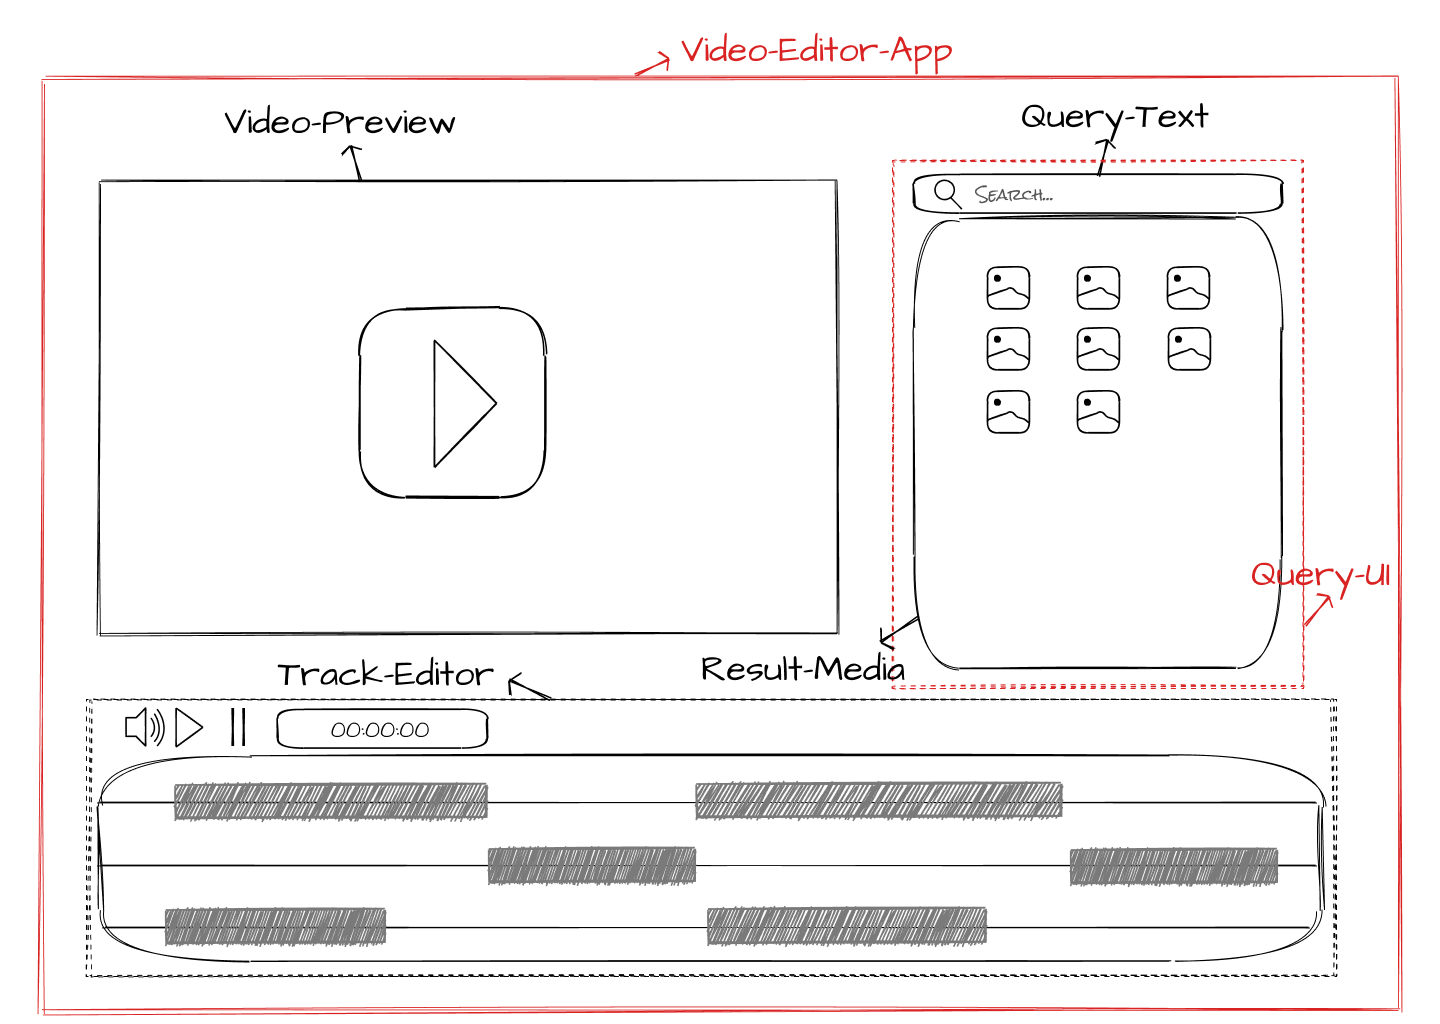
\includegraphics[width=1\textwidth]{images/Wireframe.png}
\caption{Application Mock-up}
\label{fig:appMockUp}
\end{figure}

Each of these components will be explained in more details in the next sections. 

Another important aspect regards the organizational choices. That is, the way the repository is organised, how the code structure is made, how the build and deploy phases are designed.

Firstly, components were designed to be independent and therefore, they can reside within separate online repositories. From a practical point of view, after some development iterations, an alternative approach was adopted. A monorepo\footfullcite{atlassian} setup was undertaken with the help of the Lerna\footfullcite{lerna} library. Monorepo is a repository which contains a number of projects inside the same centralized container. Since the components are used as dependencies which are injected or arranged into an application, this helps to organise and speed up the development. Nevertheless, nothing prevents from extracting components into separate repositories anytime.

\begin{figure}[H]
\centering
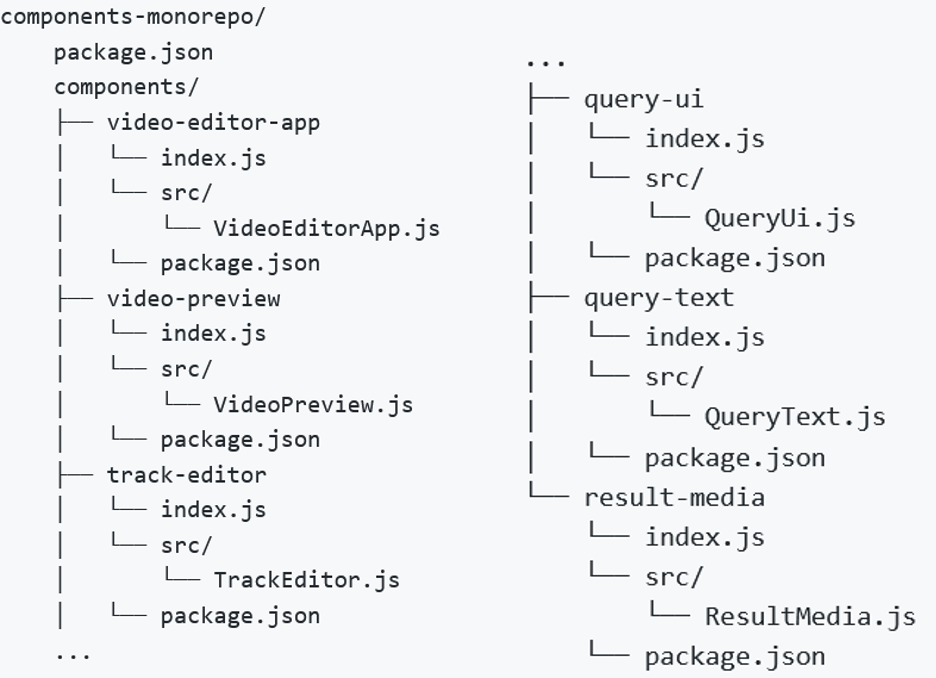
\includegraphics[width=0.8\textwidth]{images/repository.png}
\caption{Project repository structure}
\label{fig:repoStructure}
\end{figure}

The figure \ref{fig:repoStructure} shows a flat structure of components, although they can be dependent on one other. For example, Query-Ui can depend upon Query-Text specifying the latter as a project dependency inside its “package.json”. By adopting a monorepo structure the dependencies are always at hand, ready to be modified and at the same time they maintain their own commit history. Lerna is a tool that further optimizes this workflow. Among the most prominent features, it allows for dependency hoisting, versioning with the possibility of publishing components into registries like npm, and many others.

In addition, the repository structure is well suited for automation. In particular, the “index.js” file provides an entry point for every component. In this context JavaScript module bundlers can be easily implemented.
\\
\begin{lstlisting}[caption={Component entry point example},label={componentEntrypoint}, language=JavaScript]
import { QueryText } from "./src/QueryText.js";
window.customElements.define("query-text", QueryText);
\end{lstlisting}

The figure above depicts the Query-Text component although its structure is identical for every other component. Again, the objective is to offer a robust way of distributing the application as a whole and a future-proof structure for project evolution. Indeed, the last step of a development iteration in the software world is usually informally referred to by the colloquial expression “going to production”. The practical meaning is about publishing the code to the server and therefore offering it to the final users. At this point the common wish is to have the most optimized code possible. In the web development scenario this can be done with the help of module bundlers. Among prominent features, they allow to resolve dependencies, produce module maps for efficiency, and subsequently minify all the code.

Finally, several dependencies providing additional features are shared by all the components, therefore they will not be included in the descriptions contained in the next paragraphs. The dependencies were chosen and adopted following the Open Web Components initiative\footfullcite{openWC} indications. Their mission is to provide a list of best practices and recommendations for developing and sharing Web Components.

Therefore, a brief list of development dependencies is included in the project. Firstly, the purpose is indicated followed by a tool or a list of tools names and their brief description.

\begin{itemize}
\item Linting and Code checking: ESLint\footfullcite{esLint}, Prettier\footfullcite{prettier}. 
    \begin{itemize}
        \item These tools allow to keep consistent code formatting styles and avoid the most common problems by performing a statical code analysis.
    \end{itemize}
\item Testing: Karma\footfullcite{karma}, Mocha\footfullcite{mocha}.
    \begin{itemize}
        \item Testing environment for unit testing, integration testing and mocking.
    \end{itemize}
\item Interactive documentation: Storybook\footfullcite{storybook}
    \begin{itemize}
        \item It allows to visually describe the components with all the states they can assume.
    \end{itemize}
\item Building and deployment: Rollup\footfullcite{rollup}
    \begin{itemize}
        \item JavaScript module bundler used for library or application deployment.
    \end{itemize}
\end{itemize}

The next paragraphs introduce and briefly explain each component. The goal is to provide the core information about their structure and present some of the most interesting challenges encountered during development. Therefore, the next sections are not intended as a software documentation guiding through all the processes from installation to deployment. The documentation can be found by following each component’s links or by exploring the project’s root repository\footfullcite{rmxRepo}.

\section{Searching and displaying results}
\label{sec:searchingResults}

Searching and displaying the retrieved results can be considered pivotal for applications whose success can be largely measured in terms of the quantity and the quality of offered resources. Consequently, the main benefits that come from a good implementation might involve improved content discoverability and better user engagement.

These objectives were pursued by developing three components. First, a component called Query-Ui\footfullcite{rmxQueryUI} will be introduced. It is a connector between the client and server side and can be seen as a top level wrapper governing the functionalities below, of its children’s components. Indeed, it instantiates two components: Query-Text, which manages the search and autocomplete feature while Result-Media is concerned with the rendering of results found.
Notably, Query-Ui manages all the logic and information flow coming from the instantiated components. It also sends and receives data from external APIs, thereby passing data “downwards”, to the wrapped components.

An example of this relationship can be seen in the Code below.
\\
\begin{lstlisting}[caption={Query-Ui component instantiation},label={queryUi}, language=HTML5]
<query-ui>
  <query-text 
  .dictionaries=${this.dictionaries} placeholder=${this.placeholder}>
  </query-text>
  <result-media 
  .answerSet=${this.searchResults} headerTitle=${this.headerTitle}>
  </result-media>
</query-ui>
\end{lstlisting}

In this simplified example taken from one of the possible application configurations, properties and attributes are passed down to the components. Continuing with this practical example, Query-Ui internally makes an API call to the server side. In return, the endpoint responds with a dictionary – a list of words that can be autocompleted – which can be then passed to the search component. Namely, Query-Text. The principles guiding the de facto search feature are similar. The difference in implementation regards the presence of an event listener which is triggered every time users make a search. Ultimately, the results generated from the server are passed to the result viewer component, via the “answerSet” property, which renders them.

\subsection{Search component}
\label{subsec:searchComponents}

The Search component, named “Query-Text”\footfullcite{rmxQueryText} provides search and autocomplete functionalities within multi-keyed dictionaries of strings.

The idea behind Query-Text was to create a “google-like” search functionality based on lists of keywords. This is done by providing a list of prefixed dictionaries during the component instantiation. The component extracts keys from the dictionary and uses them as prefixes for autocompletion purposes. An example of valid dictionaries – not to be confused with dictionary data structures present in many programming languages – is exemplified the Code below.
\\
\begin{lstlisting}[caption={Dictionaries examples},label={dicts}, language=JavaScript, numbers=none]
{
    "filmmaker:":
        ["Martin Scorsese", "Ridley Scott", "Woody Allen", ...]
    "#:":
        ["goat", "chair", "mountain", ...]
    ...
}
\end{lstlisting}

In this example, two prefixes are present: “filmmaker:” and "\#". When users start typing one of the recognised prefixes, autocompletion based on that prefixed list of strings will be proposed. For example, by typing “\#:mou” a suggestion for the word “mountain” will be made.

Finally, by pressing the “ENTER” key or alternatively by clicking on the search button (if present), the component emits an event (through Custom Event bubble\footfullcite{mdnEvBubble}) with the actual value of the query string. An important feature is implemented to provide “fuzzy search” with autocompletion when user types into the search bar. Fuzzy search allows to tackle the possibility of typing errors made by users. A configurable options list is implemented with a scoring system offered by "Fuse.js" library\footfullcite{fuse}. Indeed, for example, if the word “montan” is typed, the user will be offered the “mountain” suggestion.

\begin{figure}[H]
\centering
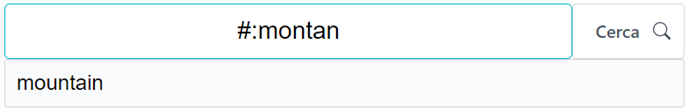
\includegraphics[width=0.8\textwidth]{images/autosuggest.png}
\caption{Query-Text autosuggestion feature}
\label{fig:queryTextAutosuggest}
\end{figure}

One of the possible issues that could arise regards the component performances. Especially when included within a more complex application, a performance-related issue emerges when users start to type fast onto the search bar. This implies the generation of a large number of DOM events and API calls if users decide to search the typed text. This issue was tackled by implementing a “debounce”\footfullcite{cssTricks} technique which limits the quantity of processed events. With configurable parameters, this instructs the autocomplete function to wait some arbitrary period of time in the order of milliseconds before taking any further action. Namely, it suggests words from the dictionary or sends the searched text to the search engine via API.

Finally, two examples of Query Text are exemplified in the figures below.

\begin{figure}[H]
\centering

\includegraphics[width=0.8\textwidth]{images/QueryText.png}
\caption{Query-Text base class}
\label{fig:queryTextBase}
\end{figure}

\begin{figure}[H]
\centering

\includegraphics[width=0.8\textwidth]{images/QueryTextSlotted.png}
\caption{Query-Text with slotted search button}
\label{fig:queryTextSlotted}
\end{figure}

The Figure \ref{fig:queryTextBase} shows the bare minimum component. Secondly, the figure \ref{fig:queryTextSlotted} shows an example of a button instantiated within the Query-Text slot.

\subsection{Results viewer component}
\label{subsec:resultsComponents}

As the name suggests, the Result-Media component renders some results onto the interface. For this project, search results are displayed as a gallery of thumbnails allowing for content selection and discovery. Importantly, the figures – or cards, as they are commonly called across UI libraries – can be dragged away from the component. This feature enables many possibilities as explored more in detail when introducing the Track-Editor component. Specifically, with the help of the native Drag and Drop API\footfullcite{mdnDnD} some information about the object can be transferred through the drop event.

The adopted preview style can be seen in the Figure \ref{fig:mediaResults} \emph{Result-Media example}.

\begin{figure}[H]
\centering
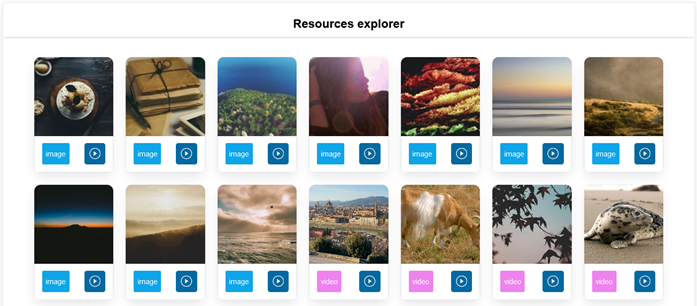
\includegraphics[width=1\textwidth]{images/ResultsMedia.png}
\caption{Result-Media example}
\label{fig:mediaResults}
\end{figure}

As mentioned before, these figures can be dragged and dropped to any valid drop target. Indeed, when users start dragging an object from the gallery,an event is triggered. This event is connected to the creation of a DataTransfer object\footfullcite{mdnDataTransf} containing all the necessary information to be transferred. For example, dragging a thumbnail that represents a video implies the insertion of the video duration onto the transferred data object. The latter can be read once the dragged item is dropped.

Additional features can also be optionally enabled. Since image thumbnails might not always be self-explanatory, the tooltip feature is also implemented in this project. Users can find further details about the resource by “hovering” on top of each media result. Continuing with the video result example, a tooltip may contain information about its title, duration, etc. Lastly, users might also be interested in reproducing the media directly inside the application. This is done by pressing the “play” button in combination with the Video-Player component which will be discussed in \ref{subsec:mediaPreview} \emph{Media Preview component}.

\section{Multimedia Editor}
\label{sec:multimediaEditor}

The most characterizing piece of this project is the Multimedia Editor. It is a top level wrapper that orchestrates the application specific behaviour. The Multimedia Editor is called “Video-Editor-App” in the project repository but by design it should be re-named and configured in relation to the application purpose. In this case, it instantiates the Track-Editor and the Video-Preview components.

As a result, the application allows to combine and arrange image, sound, and video resources by dragging them from the Result-Media component into an interactive track. Subsequently, the elements arranged in the track can be viewed inside a player and potentially exported with the help of a back end infrastructure. Although combine and preview operations are the concern of the respective components, the Multimedia Editor has a key role in making them work together. Similarly to Query-Ui, it can communicate with the outside world through APIs.

The following markup reflects the relationship between components.
\\
\begin{lstlisting}[caption={Video-Editor-App component instantiation},label={videoAppComp}, language=HTML5]
<video-editor-app>      
      <video-preview
        .resources=${this.resources}
        .singleMediaPreview=${this.singleMediaPreview}
        .executeSegmentsPreview=${this.playSegments}
        .terminateSegmentsPreview=${this.endSegments}
      ></video-preview>
      <query-ui></query-ui>
      <track-editor
        draggedElementType=${this.draggedElementType}
      ></track-editor>
</video-editor-app>
\end{lstlisting}

The figure shows some of the properties that are used for synchronising the Track-Editor with its preview. As a matter of fact, the Video-Editor-App also manages the data flow originated from the Track-Editor. This cannot be seen in the markup because of the already mentioned design decision: “data can be passed top-down through properties and can be lift-up through Custom Events”. The latter explains the logic behind the interaction. This can be further demonstrated with the help of a practical example.

A frequent scenario involves users that compose multimedia resources inside the editing track by dropping them from the content library of choice. At any moment it is possible to reproduce the arrangements made within Track-Editor component. At this point, the latter component sends an event upwards. This event is composed of a list of media elements – alongside information about their start and end dates – that were present inside the track at the exact time the “play” button was pressed. This information is captured by the Video-Editor-App whose job is to request media from external APIs. Lastly, when a successful response is available, the data is passed through to the Video-Preview, ready to be played. This behaviour will be discussed in further detail in the next sections.

\subsection{Track Editor component}
\label{subsec:trackEditpr}

“Track-Editor”\footfullcite{rmxTrackEdtior} is the most complex component created for this project application. It offers the core feature of arranging media content similarly to the way it is implemented by some of the alternative software for video-editing. Its peculiarity is that it offers this functionality directly from the browser level.

In detail, Track-Editor can be composed of multiple tracks. Depending on the configuration, an arbitrary number of tracks can be used. Tracks refer to specific media types, for example: an audio, video, and image track. Every track has a temporal dimension which allows to perform some basic operations that are key for any editing tool. Indeed, a temporal marker is also implemented for keeping track of the currently reproduced media. This can be seen in the example below:

\begin{figure}[H]
\centering
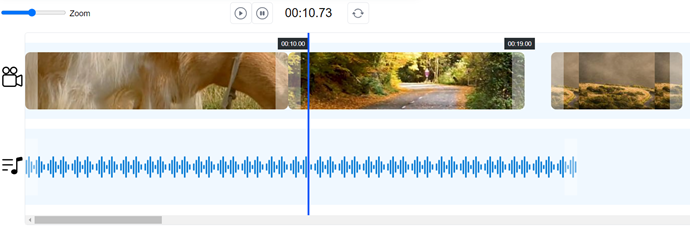
\includegraphics[width=1\textwidth]{images/TrackEditor.png}
\caption{Track-Editor example}
\label{fig:trackEditor}
\end{figure}

Currently, the Track-Editor also allows to:

\begin{itemize}
\item Receive dragged media from the application library.
\item Arrange media elements inside the tracks by dragging them back and forth.
\item Resize or trim media in relation to their type.
\item Dynamically zoom in and out the track and re-dimension all the content inside of it.
\item Check whether a specific track can contain the dragged media type.
\item Play, pause, and reset the media reproduction.
\item Open a context menu for removing undesired media.
\end{itemize}

Some interesting points can be made from this list. First of all, operating with a content length of a few seconds is different from content whose duration might be in order of several minutes. This potential problem is mitigated by the zooming functionality. Also, some basic form of error prevention has been made to preserve the preview functionality. This is done by generating an informative message on the UI stating that a specific media type cannot be put inside a track.

Finally, the ability of playing, stopping, and resetting the current tracks state is synchronized with the temporal marker – namely, the blue line in \ref{fig:trackEditor} \emph{Track-Editor example}.

From the implementation perspective, when users press play, a Custom Event is dispatched. This event can be captured thanks to its bubble property, as showed in the Code below. 
\\
\begin{lstlisting}[caption={Track-Editor event dispatch},label={customEvent}, language=JavaScript]
function dispatchEventForPreview() {
    const event = new CustomEvent('track-elements', {
      detail: {
        trackElements: this.segmentsOnTracks,
      },
      bubbles: true,
      composed: true,
    });
    this.dispatchEvent(event);
  }
\end{lstlisting}

This event transfers the current state of the Track-Editor. At a later stage this event can be captured and used for generating API requests.

\subsection{Media Preview component}
\label{subsec:mediaPreview}

The final part of this application is the media preview. The component that manages the preview is called “Video-Preview”\footfullcite{rmxVideoPreview}. As discussed in the previous paragraph, its main purpose consists in reproducing a synchronised preview of the media from the Track-Editor. Generally speaking, it can preview any number of media content, starting from a single preview to a large number of media with different media types.

An interesting implementation choice can be derived from the synchronization feature. It might be argued that the component has intuitively some sort of an internal clock or at least some way of keeping track of the elapsed time. As a matter of fact, in this case this is not entirely true. Contrary to the Track-Editor, which implements an internal timer that guides the component state. It turns out that Video-Preview does not necessarily need one. And yet it works. Walking through an example may effectively demonstrate how things work internally. Before jumping into the example, a possible way of instantiating the component is presented in the Code below.
\\
\begin{lstlisting}[caption={Video-Preview component instantiation},label={videoPreview}, language=HTML5]
<video-preview
        ?displayLoadingScreen=${this.displayLoadingScreen} 
        ?stopPlayer=${this.stopPlayer}
        ?resumePlayer=${this.resumePlayer}
        .resources=${this.resources}
        .executeSegmentsPreview=${this.playSegments} 
        .terminateSegmentsPreview=${this.endSegments}
></video-preview>
\end{lstlisting}

In particular, the “resources” property contains all the media items to be previewed. Hence, a video would be inserted into a HTML video source tag, an image would reside within an HTML img source and so on.

Assuming the scenario of Track-Editor interaction with the Video-Preview component, after putting an arbitrary number of media elements inside the tracks, the user presses the “play” button. Subsequently the following steps occur:

\begin{enumerate}
  \item All the media references are sent through a Custom Event.
  \item The Event is captured by the top level Video-Editor-App component. It requests all the items using API calls.
  \item The responses arrive asynchronously and are sent to the Video-Preview component for preview.
  \item Track-Editor starts its internal timer and checks if at the time 00:00:00 (in the minutes/seconds/milliseconds format) any media element has been positioned into the track. If yes, the next step is executed, otherwise the timer runs until it encounters an element on the track.
  \item Track-Editor emits the “executeSegmentsPreview” event containing one or more references to media elements that must be previewed.
  \item The Event is captured by the top level Video-Editor-App component and passed immediately to the Video Preview component.
  \item Video Preview selects the right resource(s) – from the resource list received in the step 3 – and starts the preview.
  \item Once the media element duration ends, the Track-Editor sends a “terminateSegmentsPreview” event.
  \item The Event is captured by the top level Video-Editor-App component and passed immediately to the Video Preview component.
  \item Video Preview selects the right resource(s) – from the resource list received in the step 3 – and stops the preview.
\end{enumerate}

This workflow – apart from the asynchronous API operations – happens with a near real time precision and continues as long as the user does not stop the reproduction or there are no more elements to be played on tracks.

As exemplified, the above mechanism makes the whole synchronized preview system work without the necessity of implementing additional timers. The Track-Editor governs the current items being played. By adopting this implementation, the Video-Preview component is simpler and more performant.

\section{Application examples}
\label{sec:appExamples}

The main application example is a prototype made for the \emph{PH-Remix} project. This application uses resources currently protected by copyright which belong to the Mediateca Toscana. At the time of writing, they are mainly documentaries. In this case the resources are short videos extracted from the original works. This is done by Artificial Intelligence algorithms as explained in this dissertation’s introduction. Figure \ref{fig:phRmxOverview} shows the application interface which reflects the components architecture as determined in section \ref{sec:SoftwareArchitecture} \emph{Project idea and Front End Software Architecture}.

\begin{figure}[H]
\centering
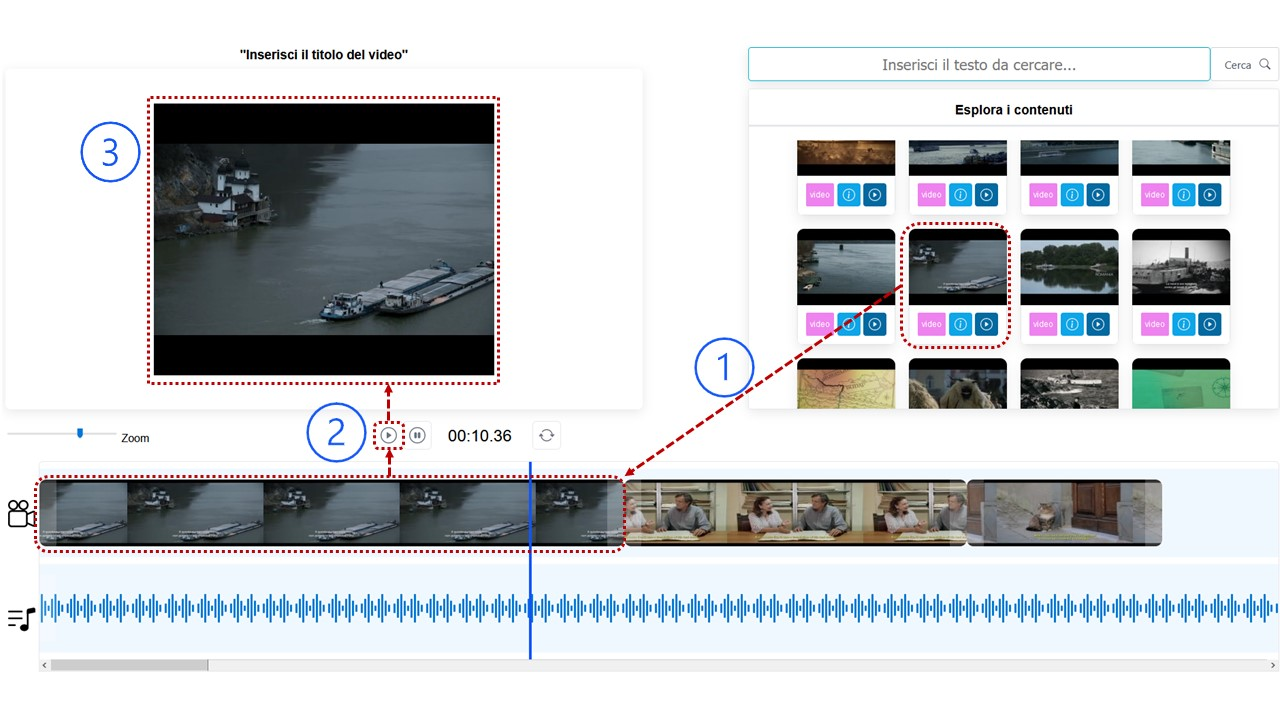
\includegraphics[width=1\textwidth]{images/PH-REmixannotatedUI.jpg}
\caption{\emph{PH-Remix} annotated User Interface}
\label{fig:phRmxOverview}
\end{figure}

Firstly, four components can be seen directly in this example. The search bar or Query-Text component is positioned in the top-right corner. Then the middle-right side shows the content library. It can be explored thanks to the thumbnails, that is representative images extracted from each video clip. This is the part managed by the Result-Media component. At the bottom there is a track editor with two different types of media tracks. A video track on top and an audio track on the bottom. This part is managed by the Track-Editor component and it allows for positioning and arranging the media from the content library. Finally, on the top-left side a preview of the content can be reproduced. The Video-Preview component is used for displaying the elements from the editing track, as well as single video clips directly from the content library.

The Figure \ref{fig:phRmxOverview} has also been annotated to show some common actions that were explained earlier in this section. There are three steps necessary to select, insert and preview the content from the library. Step 1 consists in selecting the video clip to be arranged or edited inside the track. This is done by dragging the thumbnail directly into the corresponding media track. In this case a video clip is dragged to the video track. As seen in the interface, the latter proportionally expands the thumbnail length horizontally according to the duration of the video clip. This action can be repeated for every resource in the library. Subsequently, step 2 triggers the preview of the content that was positioned on the track. This happens by pressing the “play” button above the Track-Editor. Finally, step 3 allows to preview the sequence of the arranged content. This is the most common scenario for multimedia editing and can be repeated until the desired solution is reached.

Consequently, a more fine-grained look at the interface is shown by the figure below.

\begin{figure}[H]
\centering
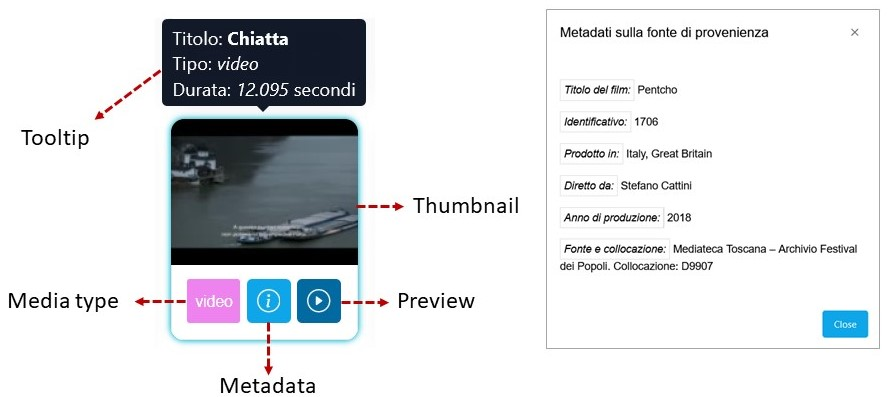
\includegraphics[width=0.8\textwidth]{images/phrDetails.jpg}
\caption{\emph{PH-Remix}: Single resource entry (on the left) and modal window with details about the resource (on the right)}
\label{fig:phRmxDetails}
\end{figure}

This shows an annotated example (from the Italian version) of a single resource entry. The left-hand side displays the element state while the cursor is "hovering" over it. When users place their cursor on top of a library element, a tooltip with some basic information appears to disambiguate the nature of the resource. In this case the thumbnail seems to depict some sort of a barge floating on water. Indeed, the tooltip describes it as a “Barge” (“Chiatta” in Italian) alongside with the media type (video) and its duration in seconds. Below the thumbnail three elements of the interface allows to perform some actions with the element. These are always visible independently from the item’s state (like the aforementioned positioning of the cursor on top of it). Going from left to right, the media type is also specified within a coloured box, with a different colour for each media type. Then in the centre some more information about the object can be shown as exemplified on the right side of Figure \ref{fig:phRmxDetails}. This is particularly useful for content with cultural value. Indeed, in this case some metadata about the extracted clip and its original source are shown. For instance, the image displays the name of the documentary, its director, year of production, physical location, etc.

The last button allows to directly preview the video clip inside the Video-Preview component. This is useful to evaluate whether the visual content of the selected items is relevant for the editing action. Then it can be dragged to the track editor, as explained above.

On the other hand, the second example is a general-purpose application which integrates the resource from the Pexels API. Although at the time of writing the User Interface is almost exactly similar to the one of the \emph{PH-Remix}, its peculiarity is that – thanks to the permissive license of the Pexels platform – it allows for legal remixing of content by everyone.
As a matter of fact, this consents unconstrained browsing of a rich Open Source catalogue of content. In particular, it consists of thousands of videos and images that can be freely built upon. Apart from the nature of the content itself, some features that are present in the \emph{PH-Remix} example are not present in the general-purpose application and vice versa. For instance the ability of viewing object metadata is relevant to cultural heritage objects, but it may not be necessary for simple pictures made for fun.  
